

% Chapter 




\chapter{Quantitative Epistemology} % Chapter title

\label{ch:quantepistemo} % For referencing the chapter elsewhere, use \autoref{ch:name} 

%----------------------------------------------------------------------------------------


\headercit{The Social Construction of What ?}{Ian Hacking}{\cite{hacking1999social}}


\bigskip

Under this provocative book title by \noun{Hacking} are implied complex mechanisms in the production of scientific knowledge. Animated debates on constructivism would be due to different metaphysical conceptions that are by essence not provable. As we have already evoked with perspectivism, scientific entreprises may have different purposes and be difficultly transferable to other contexts as we intent to do in our broad thematic vision developed in chapter~\ref{ch:thematic}.


A corollary of theoretical background proposed in chapter~\ref{ch:theory} is the need of an understanding of involved disciplines themselves to be able to build integrated heterogeneous models. The potentialities of couplings and integrations are greatly determined by existing approaches and corresponding gaps. This implies an advanced epistemological study in each field, that we propose to tackle in a systematic and quantitative way. This deliberate choice may shadow elaborated epistemological considerations but fits our purpose of preliminary investigations for the construction of models, as it may reveal investigation directions.


We describe and explore in a first section a systematic review exploration algorithm, that retrieve corpuses of references through iterative semantic extraction. We describe then briefly possible extended bibliometrics by presenting an external example of application. We finally suggest possible development directions towards unsupervised data and text-mining.






%----------------------------------------------------------------------------------------


\newpage


\section{Algorithmic Systematic Review}


\bpar{
A broad bibliographical study suggests a scarcity of quantitative models of simulation integrating both network and urban growth. This absence may be due to diverging interests of concerned disciplines, resulting in a lack of communication.  We propose to proceed to an algorithmic systematic review to give quantitative elements of answer to this question. A formal iterative algorithm to retrieve corpuses of references from initial keywords, based on text-mining, is developed and implemented. We study its convergence properties and do a sensitivity analysis. We then apply it on queries representative of the specific question, for which results tend to confirm the assumption of disciplines compartmentalization.
}{
Une étude bibliographique étendue suggère une rareté des modèles quantitatifs de simulation qui intègrent à la fois la croissance urbaine et la croissance des réseaux. Cette absence pourrait être due aux intérêts divergents des disciplines concernées qui induiraient un manque de communication. Nous proposons de procéder à une revue de la littérature systématique et algorithmique pour donner des éléments de réponse quantitatifs à cette question. Un algorithme itératif formel pour construire des corpus de références à partir de mots-clés initiaux, basé sur l'analyse textuelle, est développé et mis en oeuvre. Nous étudions ses propriétés de convergence et procédons à une analyse de sensibilité. Nous l'appliquons ensuite à des requêtes représentatives de notre question spécifique, pour lesquelles les résultats tendent à confirmer l'hypothèse d'isolation des disciplines.
}



\subsection{In search of models of co-evolution}


\bpar{
Transportation networks and urban land-use are known to be strongly coupled components of urban systems at different scales~\cite{bretagnolle2009organization}. One common approach is to consider them as co-evolving, avoiding misleading interpretations such as the myth of structural effect of transportation infrastructures~\cite{offner1993effets}. A question rapidly arising is the existence of models endogeneizing this co-evolution, i.e. taking into account simultaneous urban and network growth. We try to answer it using an algorithmic systematic review. We propose in this section, after a brief state of the art of existing literature, to present such an approach by formalizing the algorithm, which results are then presented and discussed. 
}{
Les réseaux de transport et l'usage du sol urbain sont connus pour être des composantes fortement couplées des systèmes urbains à différentes échelles~\cite{bretagnolle2009organization}. Une approche commune est de les considérer comme étant en co-évolution, tout en évitant les interprétations trompeuses comme le mythe des effets structurants des infrastructures de transport~\cite{offner1993effets}. Une question qui se présente rapidement est l'existence de modèles endogénéisant cette co-évolution, i.e. prenant en compte simultanément la croissance urbaine et celle du réseau. Nous essayons d'y répondre par une revue systématique algorithmique. Nous proposons dans cette section, après un état de l'art rapide de la littérature existante, de développer cette approche en formalisant l'algorithme, dont les résultats sont ensuite présentés et discutés.
}


\subsection{Modeling Interactions between Urban Growth and Network Growth : An Overview}

\subsubsection{Land-Use Transportation Interaction Models.}


\bpar{
A wide class of models that have been developed essentially for planning purposes, which are the so-called Land-use Transportation Interaction Models, is a first type answering our research question. See diverse reviews \cite{chang2006models}, \cite{iacono2008models} and \cite{wegener2004land} to get an idea of the heterogeneity of included approaches, that exist for more than 30 years. Recent models with diverse refinements are still developed today, such as \cite{delons:hal-00319087} which includes housing market for Paris area. Diverse aspects of the same system can be translated into many models (as \eg \cite{wegener1991one}), and traffic, residential and employment dynamics, resulting land-use evolution, influenced also by a static transportation network, are generally taken into account.
}{
Une large classe de modèle développés essentiellement dans des objectifs de planification, les modèles d'interaction entre transport de usage du sol, sont un premier type pouvant rentrer dans notre problématique. Voir les diverses revues~\cite{chang2006models},~\cite{iacono2008models} et~\cite{wegener2004land} pour avoir un aperçu de l'hétérogénéité des approches incluses, qui existent depuis plus de 30 ans. Des versions récentes avec divers raffinements sont toujours développés aujourd'hui, comme~\cite{delons:hal-00319087} qui inclut le marché immobilier pour la région parisienne. Différents aspects du même système peuvent être traduits par divers modèles (comme e.g. \cite{wegener1991one}), et le traffic, les dynamiques résidentielles et d'emploi, l'évolution de l'usage du sol en découlant, influencée aussi par un réseau de transport statique, sont généralement pris en compte.
}


\subsubsection{Network Growth Approaches}


\bpar{
On the contrary, many economic literature has done the opposite of previous models, i.e. trying to reproduce network growth given assumptions on the urban landscape, as reviewed in \cite{zhang2007economics}. In~\cite{xie2009modeling}, economic empirical studies are positioned within other network growth approaches, such as work by physicists proposing model of geometrical network growth \cite{barthelemy2008modeling}. Analogy with biological networks was also done, reproducing typical robustness properties of transportation networks \cite{tero2010rules}.
}{
A l'opposé de nombreux travaux ont pris la logique inverse, i.e. essayent de reproduire la croissance du réseau étant donné des hypothèses sur l'environnement urbain, comme résumé dans~\cite{zhang2007economics}. Dans~\cite{xie2009modeling}, les travaux économiques empiriques sont positionnés parmi les autres approches de la croissance des réseaux, comme des travaux de physiciens proposant des modèles de croissance géométrique locale~\cite{barthelemy2008modeling}. L'analogie avec la biologie a également déjà été faite, permettant de reproduire les propriétés typiques de robustesse des réseaux de transport~\cite{tero2010rules}.
}


\subsubsection{Hybrid Approaches}


\bpar{
Fewer approaches coupling urban growth and network growth can be found in the literature. \cite{barthelemy2009co} couples density evolution with network growth in a toy model. In~\cite{raimbault2014hybrid}, a simple Cellular Automaton coupled with an evolutive network reproduces stylized facts of human settlements described by Le Corbusier. At a smaller scale, \cite{achibet2014model} proposes a model of co-evolution between roads and buildings, following geometrical rules. These approaches stay however limited and rare.
}{
Peu de travaux couplant croissance urbaine et croissance du réseau sont disponibles dans la littérature. \cite{barthelemy2009co} couple l'évolution de la densité avec la croissance du réseau dans un modèle jouet. Dans~\cite{raimbault2014hybrid}, un automate cellulaire simple couplé à un réseau évolutif reproduit les faits stylisés des Etablissements Humains décrits par Le Corbusier. A une plus petite échelle,~\cite{achibet2014model} propose un modèle de co-évolution entre routes et bâtiments, en suivant des règles géométriques. Ces approches restent cependant limitées et rares.
}



\subsection{Bibliometric Analysis}


\bpar{
Literature review is a crucial preliminary step for any scientific work and its quality and extent may have a dramatic impact on research quality. Systematic review techniques have been developed, from qualitative review to quantitative meta-analyses allowing to produce new results by combining existing studies \cite{rucker2012network}. Ignoring some references can even be considered as a scientific mistake in the context of emerging information systems~\cite{lissacksubliminal}. We aim to take advantage of such techniques to tackle our issue.
Indeed, observing the form of the bibliography obtained in previous section raises some hypothesis. It is clear that all components are present for co-evolutive models to exist but different concerns and objectives seem to stop it. As it was shown by \cite{commenges:tel-00923682} for the concept of mobility, for which a ``small world of actors'' relatively closed invented a notion ad hoc, using models without accurate knowledge of a more general scientific context, we could be in an analog case for the type of models we are interested in. Restricted interactions between scientific fields working on the same objects but with different purposes, backgrounds and at different scales, could be at the origin of the relative absence of co-evolving models. 
While most of studies in bibliometrics rely on citation networks \cite{2013arXiv1310.8220N} or co-autorship networks \cite{2014arXiv1402.7268S}, we propose to use a less explored paradigm based on text-mining introduced in~\cite{chavalarias2013phylomemetic}, that obtain a dynamic mapping of scientific disciplines based on their semantic content. For our question, it has a particular interest, as we want to understand content structure of researches on the subject. We propose to apply an algorithmic method described in the following. The algorithm proceeds by iterations to obtain a stabilized corpus from initial keywords, reconstructing scientific semantic landscape around a particular subject.
}{
La revue de littérature est une étape préliminaire cruciale à toute entreprise scientifique, et sa qualité et son étendue peut avoir un impact conséquent sur le résultat final. Des techniques de revue systématique ont été développées, des revues qualitatives aux meta-analyses quantitatives qui permettent de produire des nouveaux résultats par combinaison d'études existantes~\cite{rucker2012network}. Passer sous silence certaines références peut même être considéré comme une erreur scientifique dans le contexte de l'émergence des systèmes d'information~\cite{lissacksubliminal}. Nous proposons de tirer parti de telles techniques pour traiter notre problème.
En effet, l'observation de la bibliographie obtenue dans la section précédente soulève une hypothèse. Il semble clair que toutes les briques sont présentes pour l'existence de modèles co-évolutifs mais des questionnements et objectifs différents semblent la stopper. Comme montré par~\cite{commenges:tel-00923682} pour le concept de mobilité, pour lequel un ``petit monde d'acteurs'' relativement fermé a inventé une notion ad hoc, utilisant des modèles sans connaissance préalable d'un contexte scientifique plus général, on pourrait se trouver dans un cas similaire pour le type de modèles auxquels on s'intéresse. Des interactions restreintes entre des champs scientifiques travaillant sur les mêmes objets mais avec des objectifs et contextes divergents, et à des échelles différentes, pourrait être à l'origine de l'absence de modèles co-évolutifs.
Tandis que la majorité des études en bibliométrie se reposent sur les réseaux de citation~\cite{2013arXiv1310.8220N} ou les réseaux de co-auteurs~\cite{2014arXiv1402.7268S}, nous proposons d'utiliser un paradigme moins exploré, basé sur l'analyse textuelle, introduit par~\cite{chavalarias2013phylomemetic}, qui obtient une cartographie dynamique des disciplines scientifiques en se basant sur leur contenu sémantique. La méthode est particulièrement adaptée pour notre étude puisque nous voulons comprendre la structure du contenu des recherches sur le sujet. Nous appliquons une approche algorithmique décrite par la suite. L'algorithme procède par itérations pour obtenir un corpus stabilisé à partir de mots-clés initiaux, reconstruisant l'horizon sémantique scientifique autour d'un sujet donné.
}


\subsubsection{Description of the Algorithm}


\bpar{
Let $A$ be an alphabet, $A^{\ast}$ corresponding words and $T = \cup_{k\in \mathbb{N}} {A^{\ast}}^k$ texts of finite length on it. A reference is for the algorithm a record with text fields representing title, abstract and keywords. Set of references at iteration $n$ will be denoted $\mathcal{C} \subset T^3$. We assume the existence of a set of keywords $\mathcal{K}_n$, initial keywords being $\mathcal{K}_0$. An iteration goes as follows :

\begin{enumerate}
\item A raw intermediate corpus $\mathcal{R}_n$ is obtained through a catalog request providing previous keywords $\mathcal{K}_{n-1}$.
\item Overall corpus is actualized by $\mathcal{C}_n = \mathcal{C}_{n-1} \cup \mathcal{R}_n$.
\item New keywords $\mathcal{K}_n$ are extracted from corpus through Natural Language Processing treatment, given a parameter $N_k$ fixing the number of keywords.
\end{enumerate}

The algorithm stops when corpus size becomes stable or a user-defined maximal number of iterations has been reached. Fig.~\ref{fig:quantepistemo:algo} shows the global workflow.
}{
Soit $A$ un alphabet, $A^{\ast}$ les mots correspondants et $T = \cup_{k\in \mathbb{N}} {A^{\ast}}^k$ les textes de longueur finie sur celui-ci. Ce qu'on nomme une référence est pour l'algorithme un enregistrement avec des champs textuels représentant le titre, le résumé et les mots-clés. L'ensemble de références à l'itération $n$ sera noté $\mathcal{C} \subset T^3$. Nous supposons l'existence d'un ensemble de mots-clés $\mathcal{K}_n$, les mots-clés initiaux étant $\mathcal{K}_0$. Une itération procède de la manière suivante :

\begin{enumerate}
\item Un corpus intermédiaire brut $\mathcal{R}_n$ est obtenu par une requête à un catalogue auquel on fourni les mots-clés précédents $\mathcal{K}_{n-1}$.
\item Le corpus total est actualisé par $\mathcal{C}_n = \mathcal{C}_{n-1} \cup \mathcal{R}_n$.
\item Les nouveaux mot-clés $\mathcal{K}_n$ sont extraits du corpus par Traitement du Language Naturel (NLP), étant donné un paramètre $N_k$ fixant le nombre de mot-clés.
\end{enumerate}

L'algorithme termine quand la taille du corpus devient stable ou quand un nombre maximal d'itérations défini par l'utilisateur est atteint. La figure~\ref{fig:quantepistemo:algo} montre le processus général.
}


%%%%%%%%%%%%%%%%%%%%%%%%%%%%
\begin{figure}
\centering
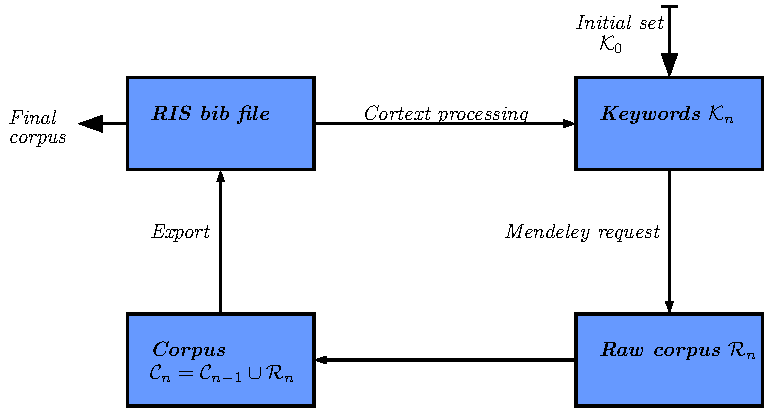
\includegraphics[width=\textwidth]{Figures/PartI/QuantitativeEpistemo/schema_algo}
\caption[Systematic review algorithm workflow]{Global workflow of the algorithm, including implementation details : catalog request is done through Mendeley API ; final state of corpuses are RIS files.}
\label{fig:quantepistemo:algo}
\end{figure}
%%%%%%%%%%%%%%%%%%%%%%%%%%%%



%%%%%%%%%%%%%%%%%%%%%%%%%%%%
\subsubsection{Results}

\paragraph{Implementation}


\bpar{
Because of the heterogeneity of operations required by the algorithm (references organisation, catalog requests, text processing), it was found a reasonable choice to implement it in Java. Source code is available on the Github repository of the project\footnote{at \texttt{https://github.com/JusteRaimbault/CityNetwork/tree/master/Models/Biblio/AlgoSR}}. Catalog request, consisting in retrieving a set of references from a set of keywords, is done using the Mendeley software API \cite{mendeley} as it allows an open access to a large database. Keyword extraction is done by Natural Language Processing (NLP) techniques, following the workflow given in \cite{chavalarias2013phylomemetic}, calling a Python script that uses \cite{bird2006nltk}.
}{
De par l'hétérogénéité des opérations requises par l'algorithme (organisation des références, requêtes au catalogue, analyse textuelle), le language Java s'est présenté comme une alternative raisonnable. Le code source est disponible sur le dépôt ouvert du projet\footnote{à l'adresse \texttt{https://github.com/JusteRaimbault/CityNetwork/tree/master/Models/Biblio/AlgoSR}}. Les requêtes au catalogue, qui consistent à récupérer un ensemble de références à partir d'un ensemble de mots-clés, sont faites via l'API du logiciel Mendeley~\cite{mendeley} qui permet un accès ouvert à une base de données conséquente. L'extraction des mots-clés est effectuée par techniques d'Analyse Textuelle (NLP) selon le processus donné dans~\cite{chavalarias2013phylomemetic}, via un script Python qui utilise~\cite{bird2006nltk}.
}


\paragraph{Convergence and Sensitivity Analysis}


\bpar{
A formal proof of algorithm convergence is not possible as it will depend on the empirical unknown structure of request results and keywords extraction. We need thus to study empirically its behavior. Good convergence properties but various sensitivities to $N_k$ were found as presented in Fig.~\ref{fig:quantepistemo:sensitivity}. We also studied the internal lexical consistence of final corpuses as a function of keywords number. As expected, small number yields more consistent corpuses, but the variability when increasing stays reasonable.
}{
Une preuve formelle de convergence de l'algorithme n'est guère envisageable puisque qu'elle dépendra de la structure empirique inconnue des résultats de requête et d'extraction de mots-clés. Il est donc nécessaire d'étudier le comportement de l'algorithme de manière empirique. Comme présenté en figure~\ref{fig:quantepistemo:sensitivity}, l'algorithme a de bonnes propriétés de convergence mais diverse sensibilités à $N_k$. Nous étudions également la cohérence lexicale interne des corpus finaux et fonction du nombre de mots-clés. Comme attendu, des valeurs faibles produisent des corpus plus cohérents, mais la variabilité lorsque qu'elles augmentent reste raisonnable.
}



%%%%%%%%%%%%%%%%%%%%%%%%%%%%
\begin{figure}
\centering
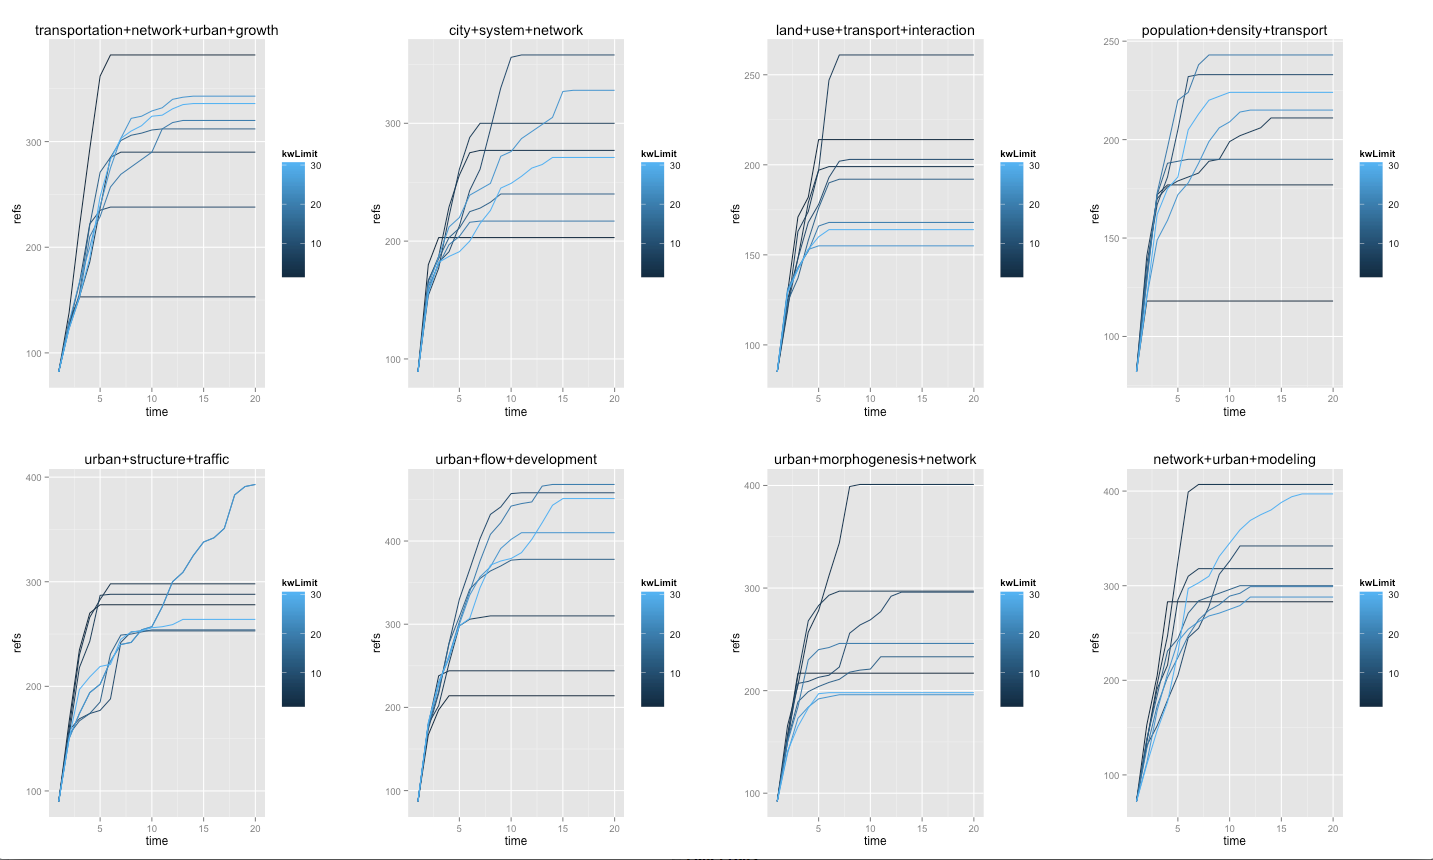
\includegraphics[width=\textwidth]{Figures/PartI/QuantitativeEpistemo/explo}
\medskip
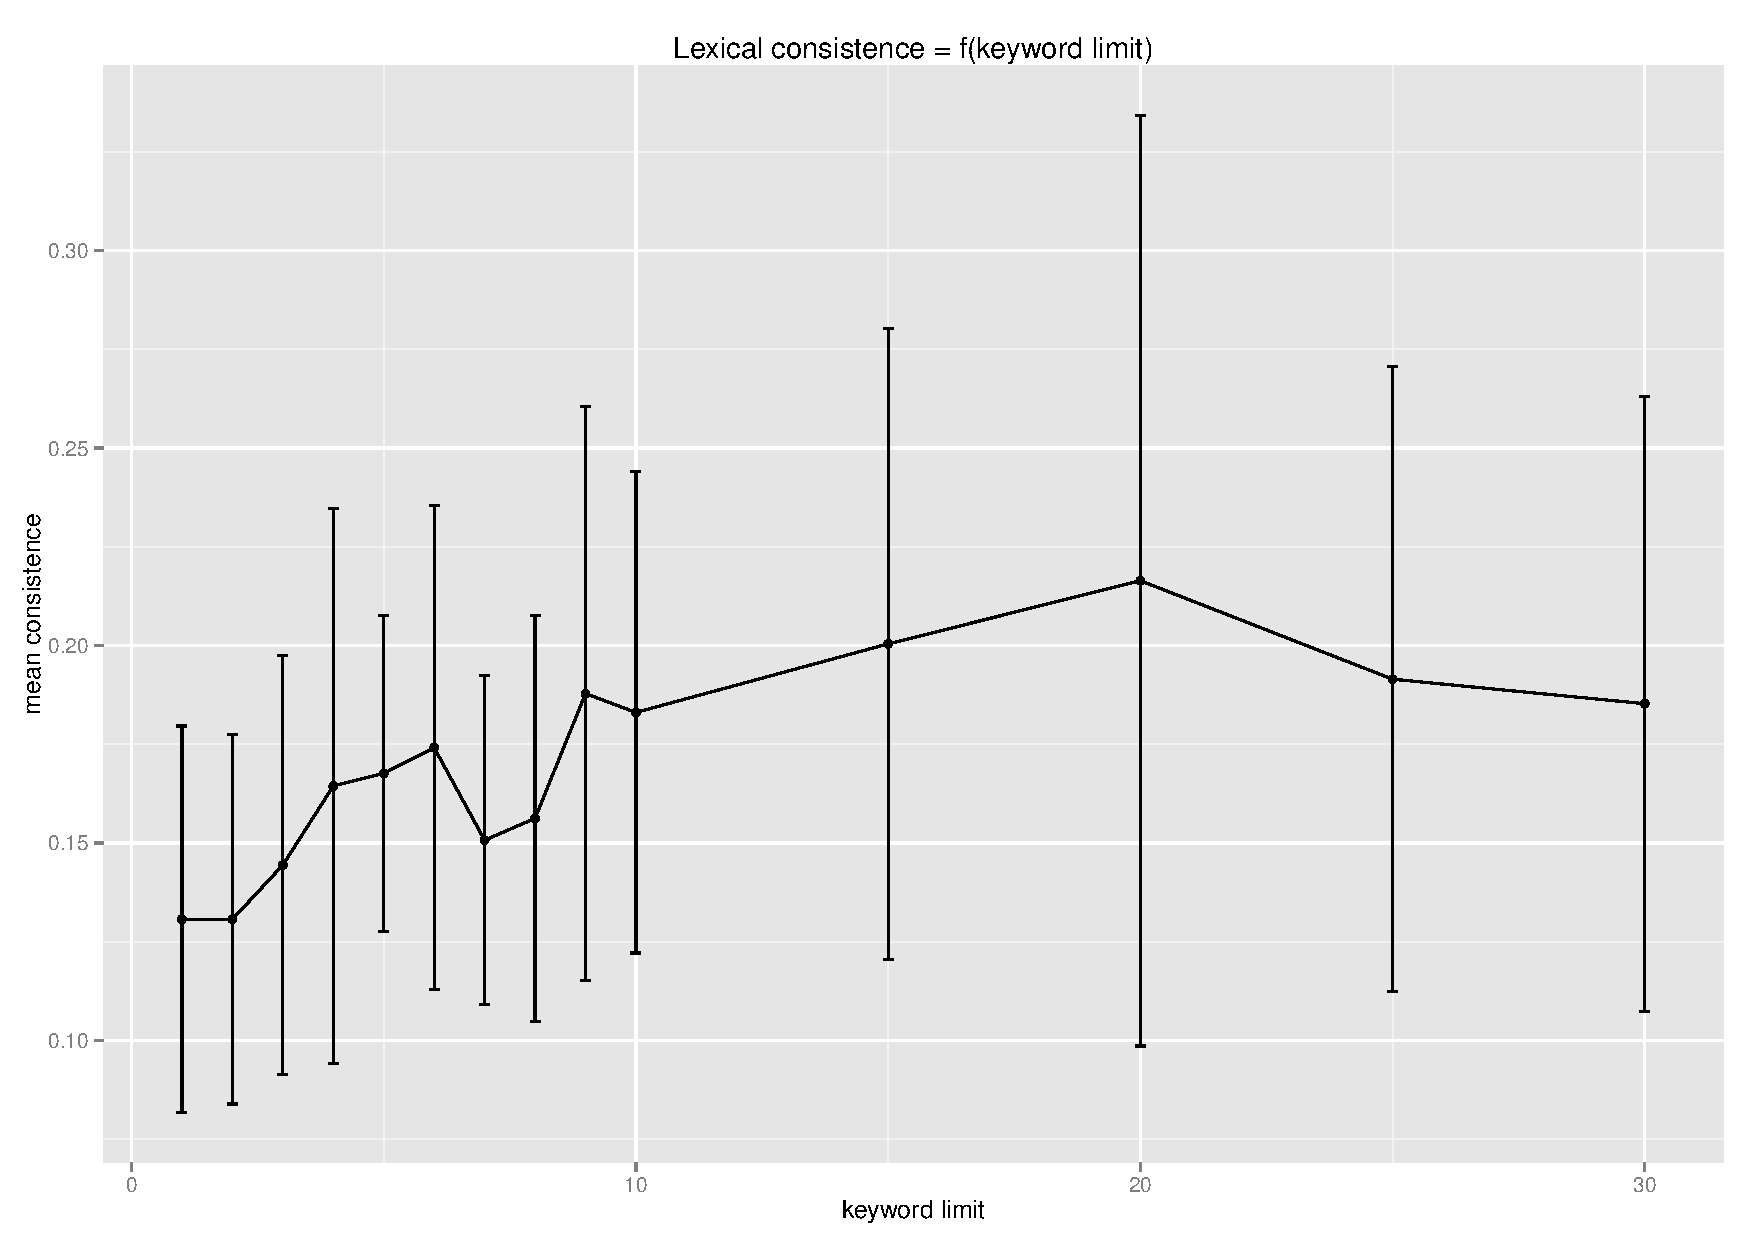
\includegraphics[width=0.8\textwidth]{Figures/PartI/QuantitativeEpistemo/lexicalConsistence_MeanSd}
\caption[Convergence and sensitivity analysis of systematic review algorithm]{Convergence and sensitivity analysis. Left : Plots of number of references as a function of iteration, for various queries linked to our theme (see further), for various values of $N_k$ (from 2 to 30). We obtain a rapid convergence for most cases, around 10 iterations needed. Final number of references appears to be very sensitive to keyword number depending on queries, what seems logical since encountered landscape should strongly vary depending on terms. Right : Mean lexical consistence and standard error bars for various queries, as a function of keyword number. Lexical consistence is defined though co-occurrences of keywords by, with $N$ final number of keywords, $f$ final step, and $c(i)$ co-occurrences in references, $k = \frac{2}{N(N-1)}\cdot \sum_{i,j \in \mathcal{K}_f}{\left| c(i) - c(j) \right|}$. The stability confirms the consistence of final corpuses.}
\label{fig:quantepistemo:sensitivity}
\end{figure}
%%%%%%%%%%%%%%%%%%%%%%%%%%%%




\bpar{
Once the algorithm is partially validated, we apply it to our question. We start from five different initial requests that were manually extracted from the various domains identified in the bibliography (that are ``city system network'', ``land use transport interaction'', ``network urban modeling'', ``population density transport'', ``transportation network urban growth''). We take the weakest assumption on parameter $N_k=100$, as it should less constrain reached domains. After having constructed corpuses, we study their lexical distances as an indicator to answer our initial question. Large distances would go in the direction of the assumption made above, i.e. that discipline self-centering may be at the origin of the lack of interest for co-evolutive models. We show in Table~\ref{tab:quantepistemo:lexical} values of relative lexical proximity, that appear to be significantly low, confirming this assumption.
}{
Lorsque l'algorithme a été partiellement validé, on peut l'appliquer à notre question. Nous partons de cinq différentes requêtes initiales qui ont été manuellement extraites des divers domaines identifiés dans la bibliographie (qui sont ``city system network'', ``land use transport interaction'', ``network urban modeling'', ``population density transport'', ``transportation network urban growth''). Nous prenons l'hypothèse la plus faible pour le paramètre $N_k=100$, au sens où les domaines atteints devraient être moins restreints. Après avoir construit les corpus, nous étudions leur cohérence lexicale comme un indicateur de réponse à notre question initiale. De grande distances devraient confirmer l'hypothèse formulée ci-dessus, i.e. que des disciplines auto-centrées pourraient être à l'origine d'un manque d'intérêt pour des modèles co-évolutifs. La table~\ref{tab:quantepistemo:lexical} montre les valeurs de la proximité lexicale relative, qui est significativement basse, confirmant notre hypothèse.
}



\begin{table}
\centering
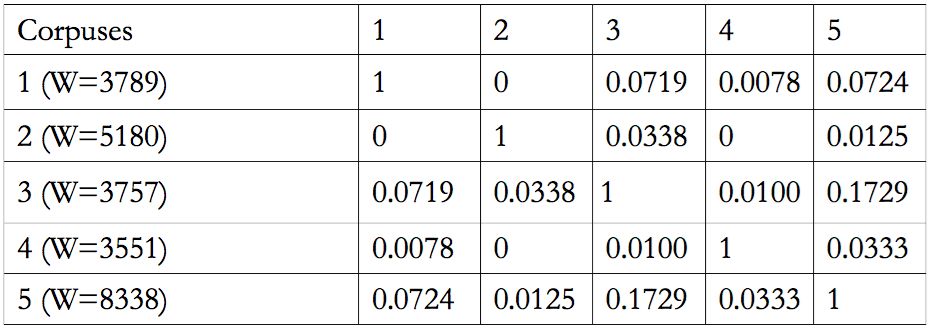
\includegraphics[width=\textwidth]{Figures/PartI/QuantitativeEpistemo/corpusesDistances}
\caption[Stationary lexical proximities]{Symmetric matrix of lexical proximities between final corpuses, defined as the sum of overall final keywords co-occurrences between corpuses, normalized by number of final keywords (100). We obtain very low values, confirming that corpuses are significantly far. Size of final corpuses is given as $W$.}
\label{tab:quantepistemo:lexical}
\end{table}



\bpar{
Possible developments can include the construction of citation networks through an automatic access to Google Scholar that provides backward citations. The confrontation of inter-cluster coefficients on the citation network for the different corpuses with lexical consistence are an essential aspect of a further validation of our results.
}{
Les développements possibles incluent la construction de réseaux de citation via un accès automatique à Google Scholar qui fournit les citations entrantes. La confrontation des coefficients inter-clusters pour le réseau de citations entre les différents corpus avec la cohérence lexicale est un aspect clé d'une validation approfondie des résultats.
}



\bpar{
The disturbing absence of models simulating the co-evolution of transportation networks and urban land-use, confirmed through a state-of-the-art covering many domain, may be due to the absence of communication between scientific disciplines studying different aspects of that problems. We have proposed an algorithmic method to give elements of answers through text-mining-based corpus extraction. First numerical results seem to confirm the assumption. However, such a quantitative analysis should not be considered alone, but rather come as a back-up for qualitative studies that will be the object of further work, such as the one lead in~\cite{commenges:tel-00923682}, in which questionnaires with historical actors of modeling provide highly relevant information.
}{
L'absence peu explicable a priori de modèles qui simulent la co-évolution des réseaux de transport et de l'usage du sol urbain, qui se confirme à première vue par un état de l'art couvrant des domaines disparates, pourrait être due à l'absence de communication entre les disciplines scientifiques étudiant différents aspects du problème. Nous avons proposé une méthode algorithmique pour donner des éléments de réponse par l'extraction de corpus basée sur l'analyse textuelle. Les premiers résultats numériques semblent confirmer l'hypothèse. Cependant, une telle analyse quantitative ne doit pas être considérée seule, mais devrait plutôt venir comme soutien à des études qualitatives qui peuvent être l'objet de développements futurs, comme celle menée dans~\cite{commenges:tel-00923682}, dans laquelle des questionnaires avec des acteurs historiques fournit des informations extrêmement pertinentes.
}




%--------------------------------------------------------------

\newpage

% Section describing cybergeo method.

\section{Refining bibliometrics through Hyper-network analysis}

%%%%%%%%%%%%%%
\subsection{Context}

As described before, semantic analysis does not contain all the information on disciplinary compartmentation nor on patterns of propagation of scientific knowledge as the ones contained in citation networks for example. Furthermore, data collection in the previous algorithm is subject to convergence towards self-consistent themes because of the proper structure of the method. It may give more insight about scientific social patterns of ontological choices in modeling to study communities in broader networks, that would more correspond to disciplines (or sub-disciplines depending on granularity level).



Previous works in quantitative epistemology using various types of networks have shown interesting potentialities. For the citation network, a good predicting power for citation patterns is for example obtained in~\cite{2013arXiv1310.8220N}. Co-authorship networks can also be used for predictive models~\cite{2014arXiv1402.7268S}. A multilayer network approach was recently proposed in~\cite{2016arXiv160106075O}, using bipartites networks of papers and scholars, in order to produce measures of interdisciplinarity. Disciplines can be stratified into layers to reveal communities between them and therein collaboration patterns~\cite{2015arXiv150601280B}. Keyword networks are used in other fields such as economics of technology~\cite{choi2014patent,shibata2008detecting}.


%%%%%%%%%%%%%
\subsection{Application to a scientific journal}

\subsubsection{Presentation}

We briefly describe here an ongoing study that implemented the ideas given above for the particular case of a scientific journal for which bibliographical data is difficult to obtain, that is \texttt{cybergeo}, an electronic journal in theoretical and quantitative geography, that is concerned with open science issues such as peer-review ethics transparency~\cite{10.1371/journal.pone.0147913}. Our approach combine semantic communities analysis (as done in~\cite{2016arXiv160208451P} but with keyword extraction ; \cite{2015arXiv151003797G} analyses semantic networks of political debates) with citation network to extract e.g. interdisciplinarity measures.

\subsubsection{Implementation}

The general architecture for data collection is presented in Fig.~\ref{fig:quantepistemo:data}. Citation data is collected from \texttt{Google Scholar}, that is the only source for incoming citations~\cite{noruzi2005google} in our case as the journal is not referenced in other databases. We are aware of the possible biaises using this single source~\cite{bohannon2014scientific}\footnote{or see \url{http://iscpif.fr/blog/2016/02/the-strange-arithmetic-of-google-scholars/}}, but these critics are more directed towards search results than citation counts. 

Text processing is done the same way as in previous section, expect that a particular treatment is done to language detection using \emph{stop-words} and a specific tagger \texttt{TreeTagger} is used for other languages than english~\cite{schmid1994probabilistic}.



%%%%%%%%%%%%%%%%%%
\begin{figure}
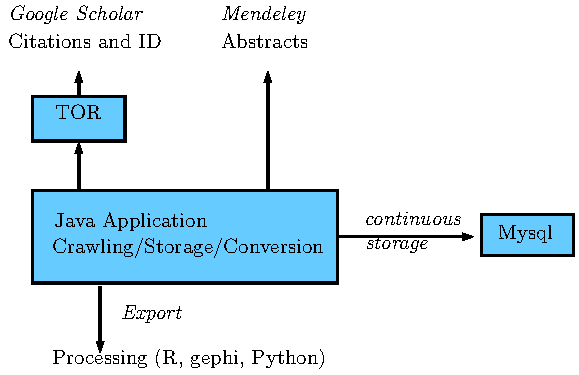
\includegraphics[width=\textwidth]{Figures/PartI/QuantitativeEpistemo/HyperNetwork/archi}
\caption[Heterogeneous Bibliographical Data Collection]{Heterogeneous Bibliographical Data Collection. Architecture of the application for content (semantic data), metadata and citation data collection.}
\label{fig:quantepistemo:data}
\end{figure}
%%%%%%%%%%%%%%%%%%


\subsubsection{Results}


We show in figures~\ref{fig:quantepistemo:citnw} and~\ref{fig:quantepistemo:semanticnw} preliminary results on citation and semantic network. We are able by the reconstruction of the citation network at depth $\pm 1$ from the original 1000 references of the journal to retrieve around $45\cdot 10^6$ references, on which $2.1\cdot 10^6$ are retrieved with abstract text allowing semantic analysis. We retrieve by community detection in the semantic network typical geographical disciplines, such as :

\begin{itemize}
\item Hydrology : \texttt{water, basin, river, capac}
\item Traffic : \texttt{traffic, road, vehicl}
\item Biogeography : \texttt{habitat, soil, veget, ecosystem}
\item Political Science : \texttt{polit, cultur, societi, debat}
\item Economy : \texttt{market, economi, privat, competit, industri}
\item Transportation : \texttt{transport, travel}
\item Teledetection : \texttt{cluster, imag, classif, satellit}
\item Education : \texttt{educ, age, student, school}
\item Health : \texttt{diseas, infect}
\item GIS : \texttt{gi, geograph inform system}
\item Social geography : \texttt{neighborhood, resid}
\end{itemize}



Distribution of keywords within reconstructed disciplines provides an article-level interdisciplinarity, and we can construct various measures at the journal level. Combination of citation and semantic layers in the hyper-network provide second order interdisciplinarity measures. The construction of null models for comparison and the collection of currently missing data (journals for other papers) are currently ongoing so these results are not presented here.



\subsection{Application}

We will try to reconstruct the same way disciplines around our thematic, and by for example identifying bridge articles (nodes with high centrality or vulnerability) identify crucial thematic elements and research directions.

\bigskip

An other application will be the reflexivity of our thesis : we attend to proceed to similar analysis on our proper bibliography (and its evolution, available via \texttt{git} history), to understand our patterns of knowledge, possible gaps or unveil unexpected developments.


%%%%%%%%%%%%%%%%%
\begin{figure}
%\hspace{-3cm}
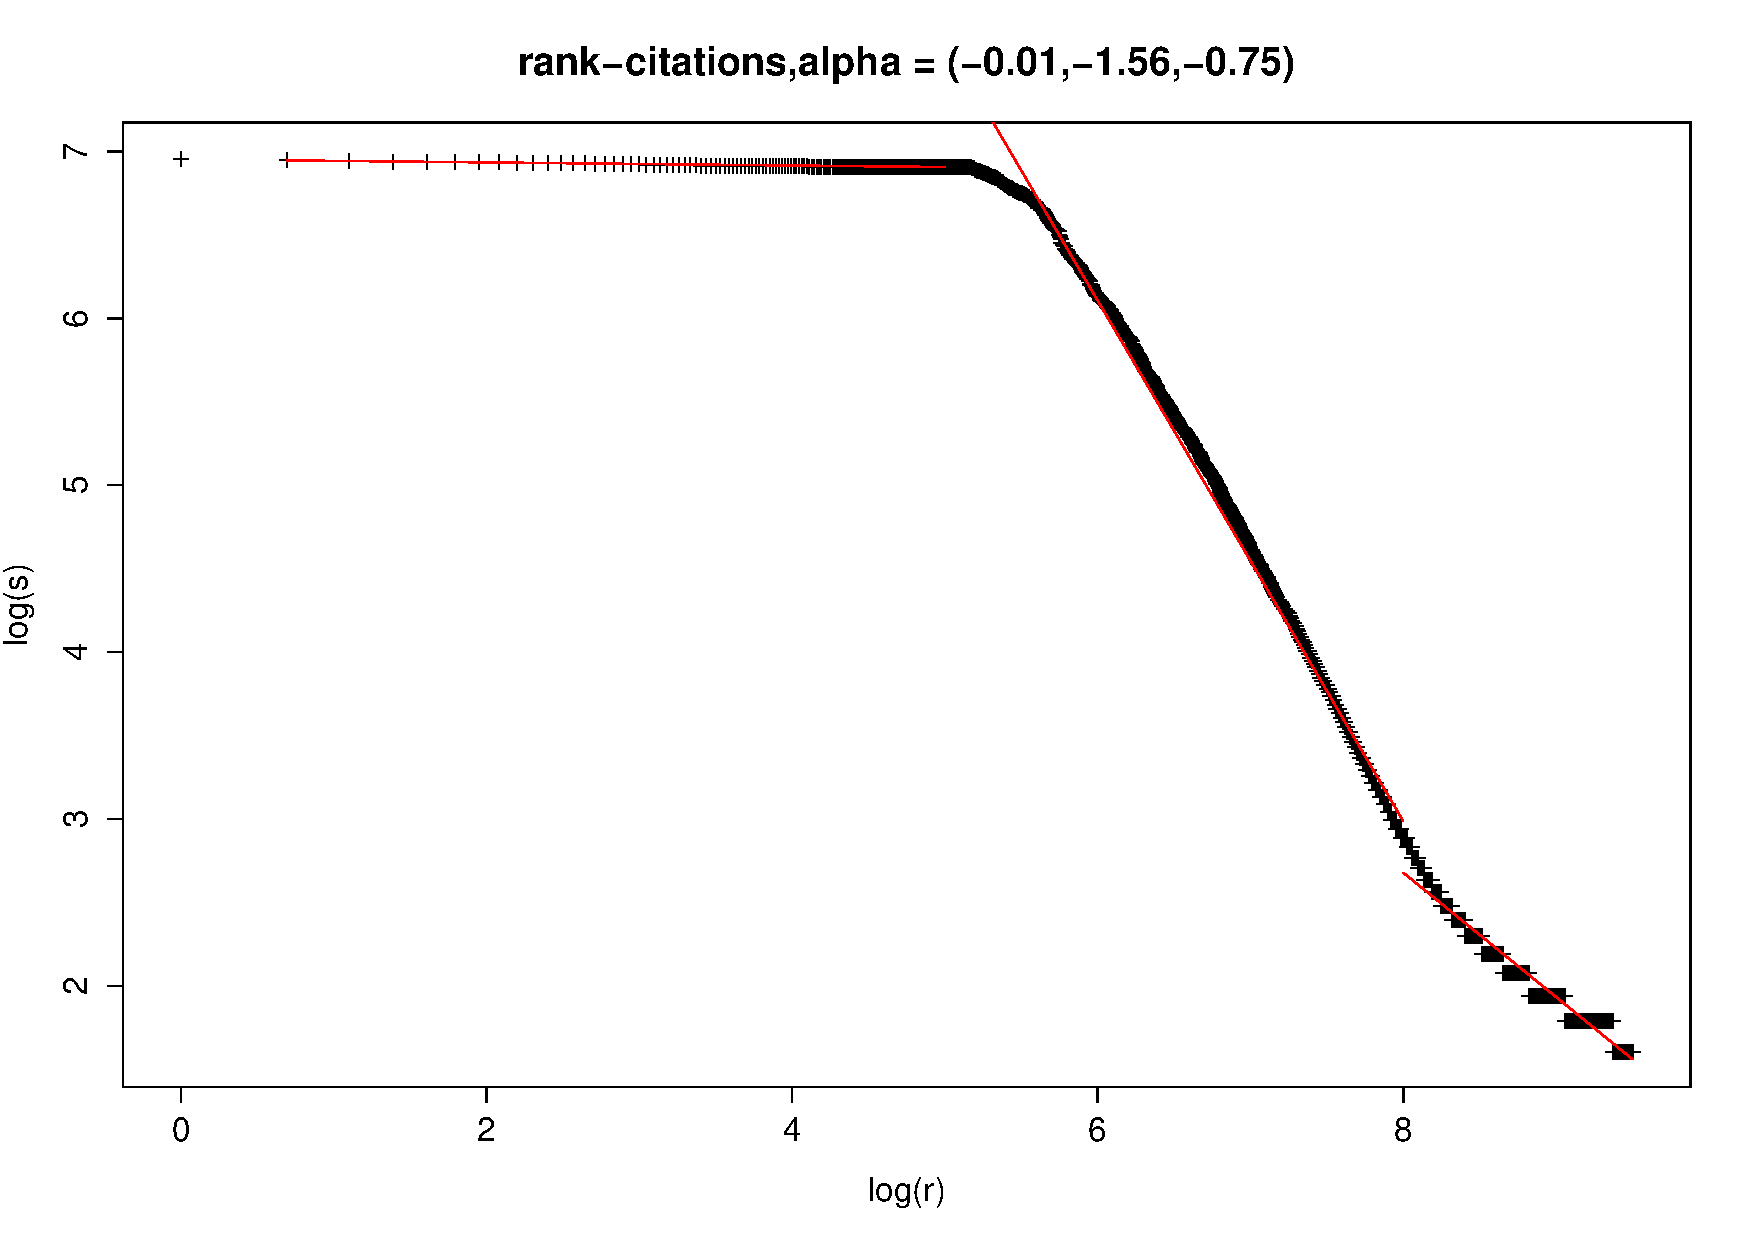
\includegraphics[width=\textwidth]{Figures/PartI/QuantitativeEpistemo/HyperNetwork/rank-size-all}
%\hspace{-3cm}
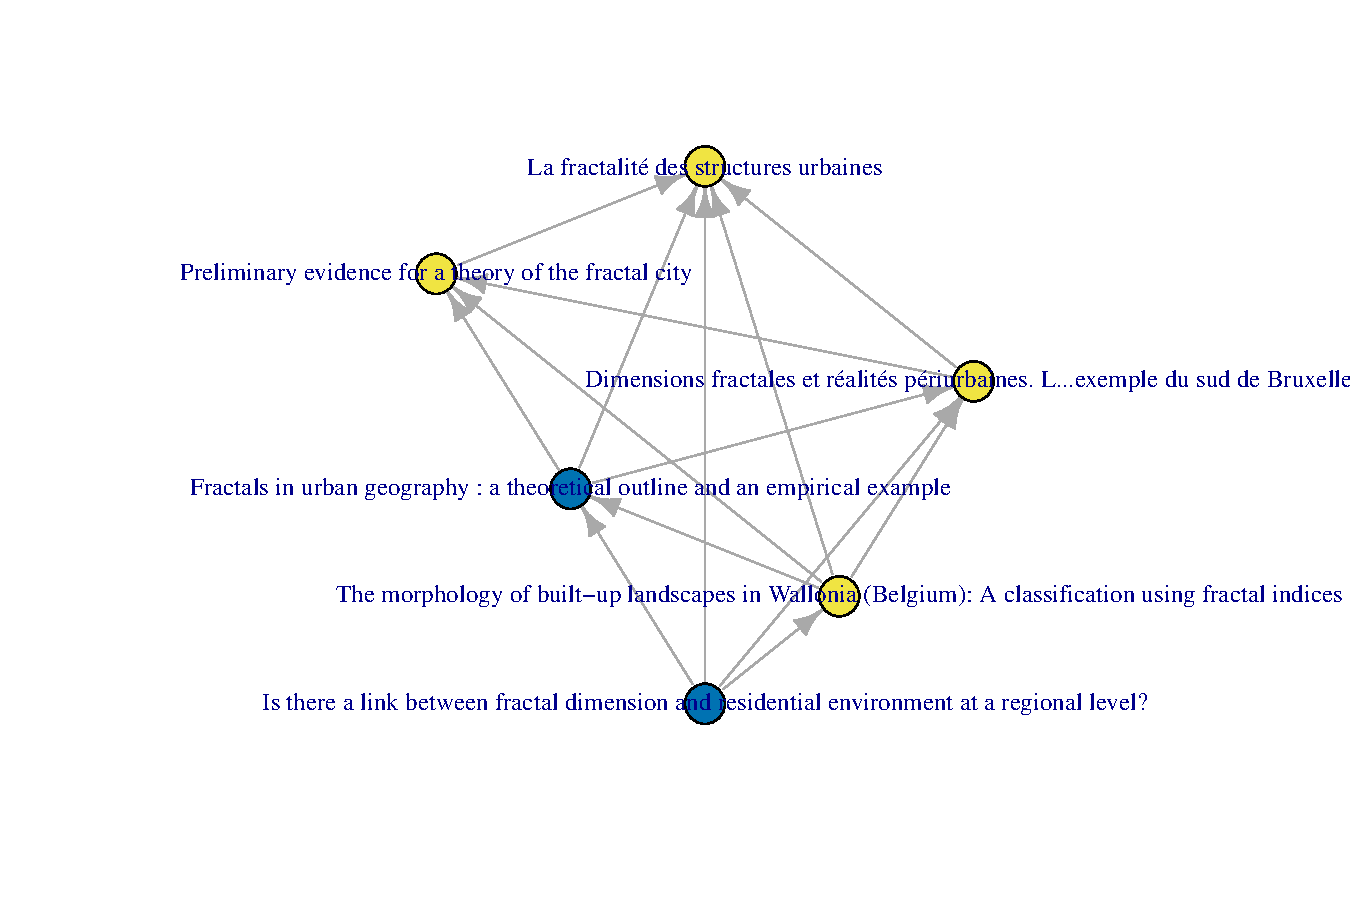
\includegraphics[width=\textwidth]{Figures/PartI/QuantitativeEpistemo/HyperNetwork/cybclic_2cyb_13761}
\caption[Properties of the citation network]{Properties of the citation network. Top : Rank-size plot of in-degrees ; three superposing successive regimes must correspond to different literature types or practices across disciplines. Bottom : example of a maximal clique in the citation network, paper of \texttt{cybergeo} being in blue.}
\label{fig:quantepistemo:citnw}
\end{figure}
%%%%%%%%%%%%%%%%%


%%%%%%%%%%%%%%%%%%
\begin{figure}
\hspace{-2cm}
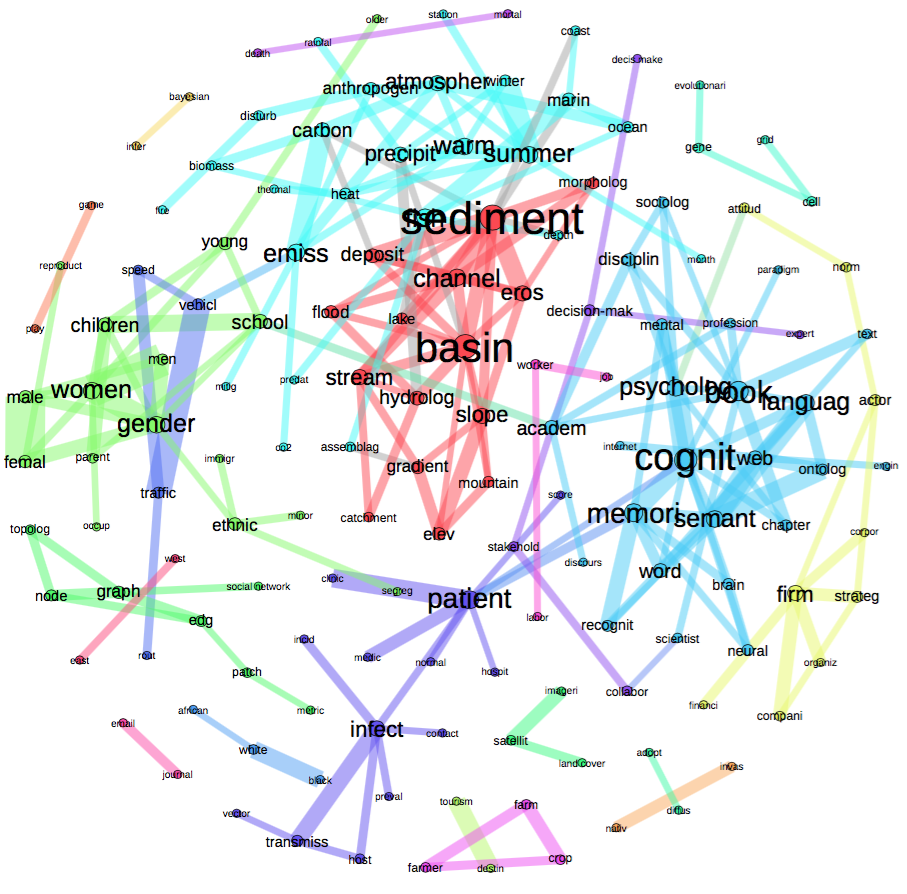
\includegraphics[width=1.4\textwidth]{Figures/PartI/QuantitativeEpistemo/HyperNetwork/all_lesslinks}
\caption[Semantic network of concepts in quantitative geography]{Semantic network of concepts in quantitative geography. Corpus consists of around $2\cdot 10^5$ abstracts of publications at a topological distance shorter than 2 from the journal \texttt{cybergeo} in the citation network. Relevance of keywords were estimated with a bootstrap method, and semantic network is constructed by co-occurrences of keywords (cut at larger degrees, 10\% here to delete hubs such as \texttt{model} or \texttt{space} and efficiently reveal communities).}
\label{fig:quantepistemo:semanticnw}
\end{figure}
%%%%%%%%%%%%%%%%%%







%--------------------------------------------------------------



\provisory{


\newpage

%  Project section : describing ideas for more advanced text mining


\section{Towards modeling purpose and context automatic extraction}


A possible direction to strengthen our quantitative epistemological analysis would be to work on full textes related to the modeling of interaction between networks and territories, with the aim to automatically extract thematics within articles. The idea would be to perform some kind of automatized modelography, with possible features to be extracted that would be ontologies, model architecture or structures, scales, or even typical parameter values. It is not clear to what degree structure of models can be extracted from their description in papers and it surely depends on the discipline considered. For example in a framed field such as transportation planning, using a pre-defined ontology (in the sense of dictionary) and a fuzzy grammar could be efficient to extract information as the discipline is relatively formatted. In theoretical and quantitative geography, beyond the barrier of language, information organisation is surely less subject to unsupervised data-mining because of the more literary nature of the discipline : synonyms and figures of speech are generally the norm in good level human sciences writing, fuzzing a possible generic structure of knowledge description. 

Depending on extended results of the two previous sections and on thematic requirements (huge need of knowledge on precise models structure, that may appear when trying to construct more specialized operational models), this project may be conducted with more or less investment.

% cit LDA for thematic extraction ?




}



